\centering

\begin{tabular}{l|cc|ccccccc} 
    \toprule
    a&b&c\\
    \midrule 
    a&b&c\\
    a&b&c\\
    \bottomrule
\end{tabular}
\vspace{0.5cm}

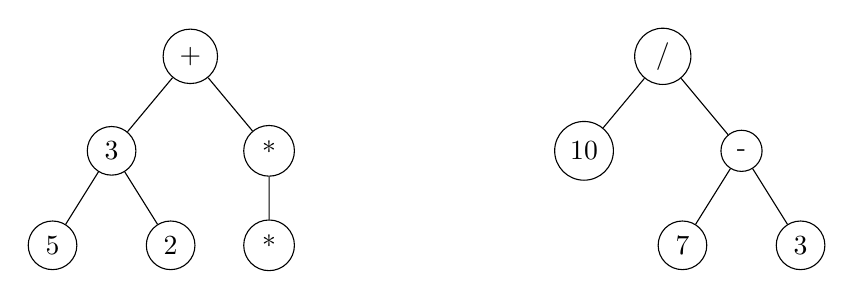
\begin{tikzpicture}[level distance=1.2cm,
    level 1/.style={sibling distance=2cm},
    level 2/.style={sibling distance=1.5cm}]

    \node[circle,draw] {+}
        child { 
            node[circle,draw] {3} 
            child { node[circle,draw] {5} }
            child { node[circle,draw] {2} }
        }
        child { 
            node[circle,draw] {*}
            child { 
                node[circle,draw] {*}
            }
        };

    \begin{scope}[xshift=6cm]

        \node[circle,draw] {/}
            child { 
                node[circle,draw] {10} 
            }
            child { 
                node[circle,draw] {-}
                child { node[circle,draw] {7} }
                child { node[circle,draw] {3} }
            };

    \end{scope}
\end{tikzpicture}